\section{Model Validation}
\label{sec:model_validation}

We validate our model in two ways: 1) We look at the in-sample fit over the estimation
period. 2) We look at the out-of-sample fit for November. The last one is a challenging
test for our model because there was a strong policy change between the estimation
period and November. The model convincingly passes both tests.


\subsection{In-Sample Fit}

Despite fitting only four free parameters, the in-sample fit is very good. The best fit
is achieved in the largest age groups. This is so mechanically, because we weight the
deviations between simulated and observed infection rates by group sizes. The worst fit
is achieved for the 80 to 100 years old. The model predicts too few infections for these
groups because they have very few contacts in all contact types we have included so far.
We plan to address this issue soon by adding another contact type that captures all
contacts in the data by \citet{Mossong2008} that we have not included so far. Moreover,
we expect an improved model fit when we allow for more free parameters.


\begin{figure}[!tp]
    \centering
    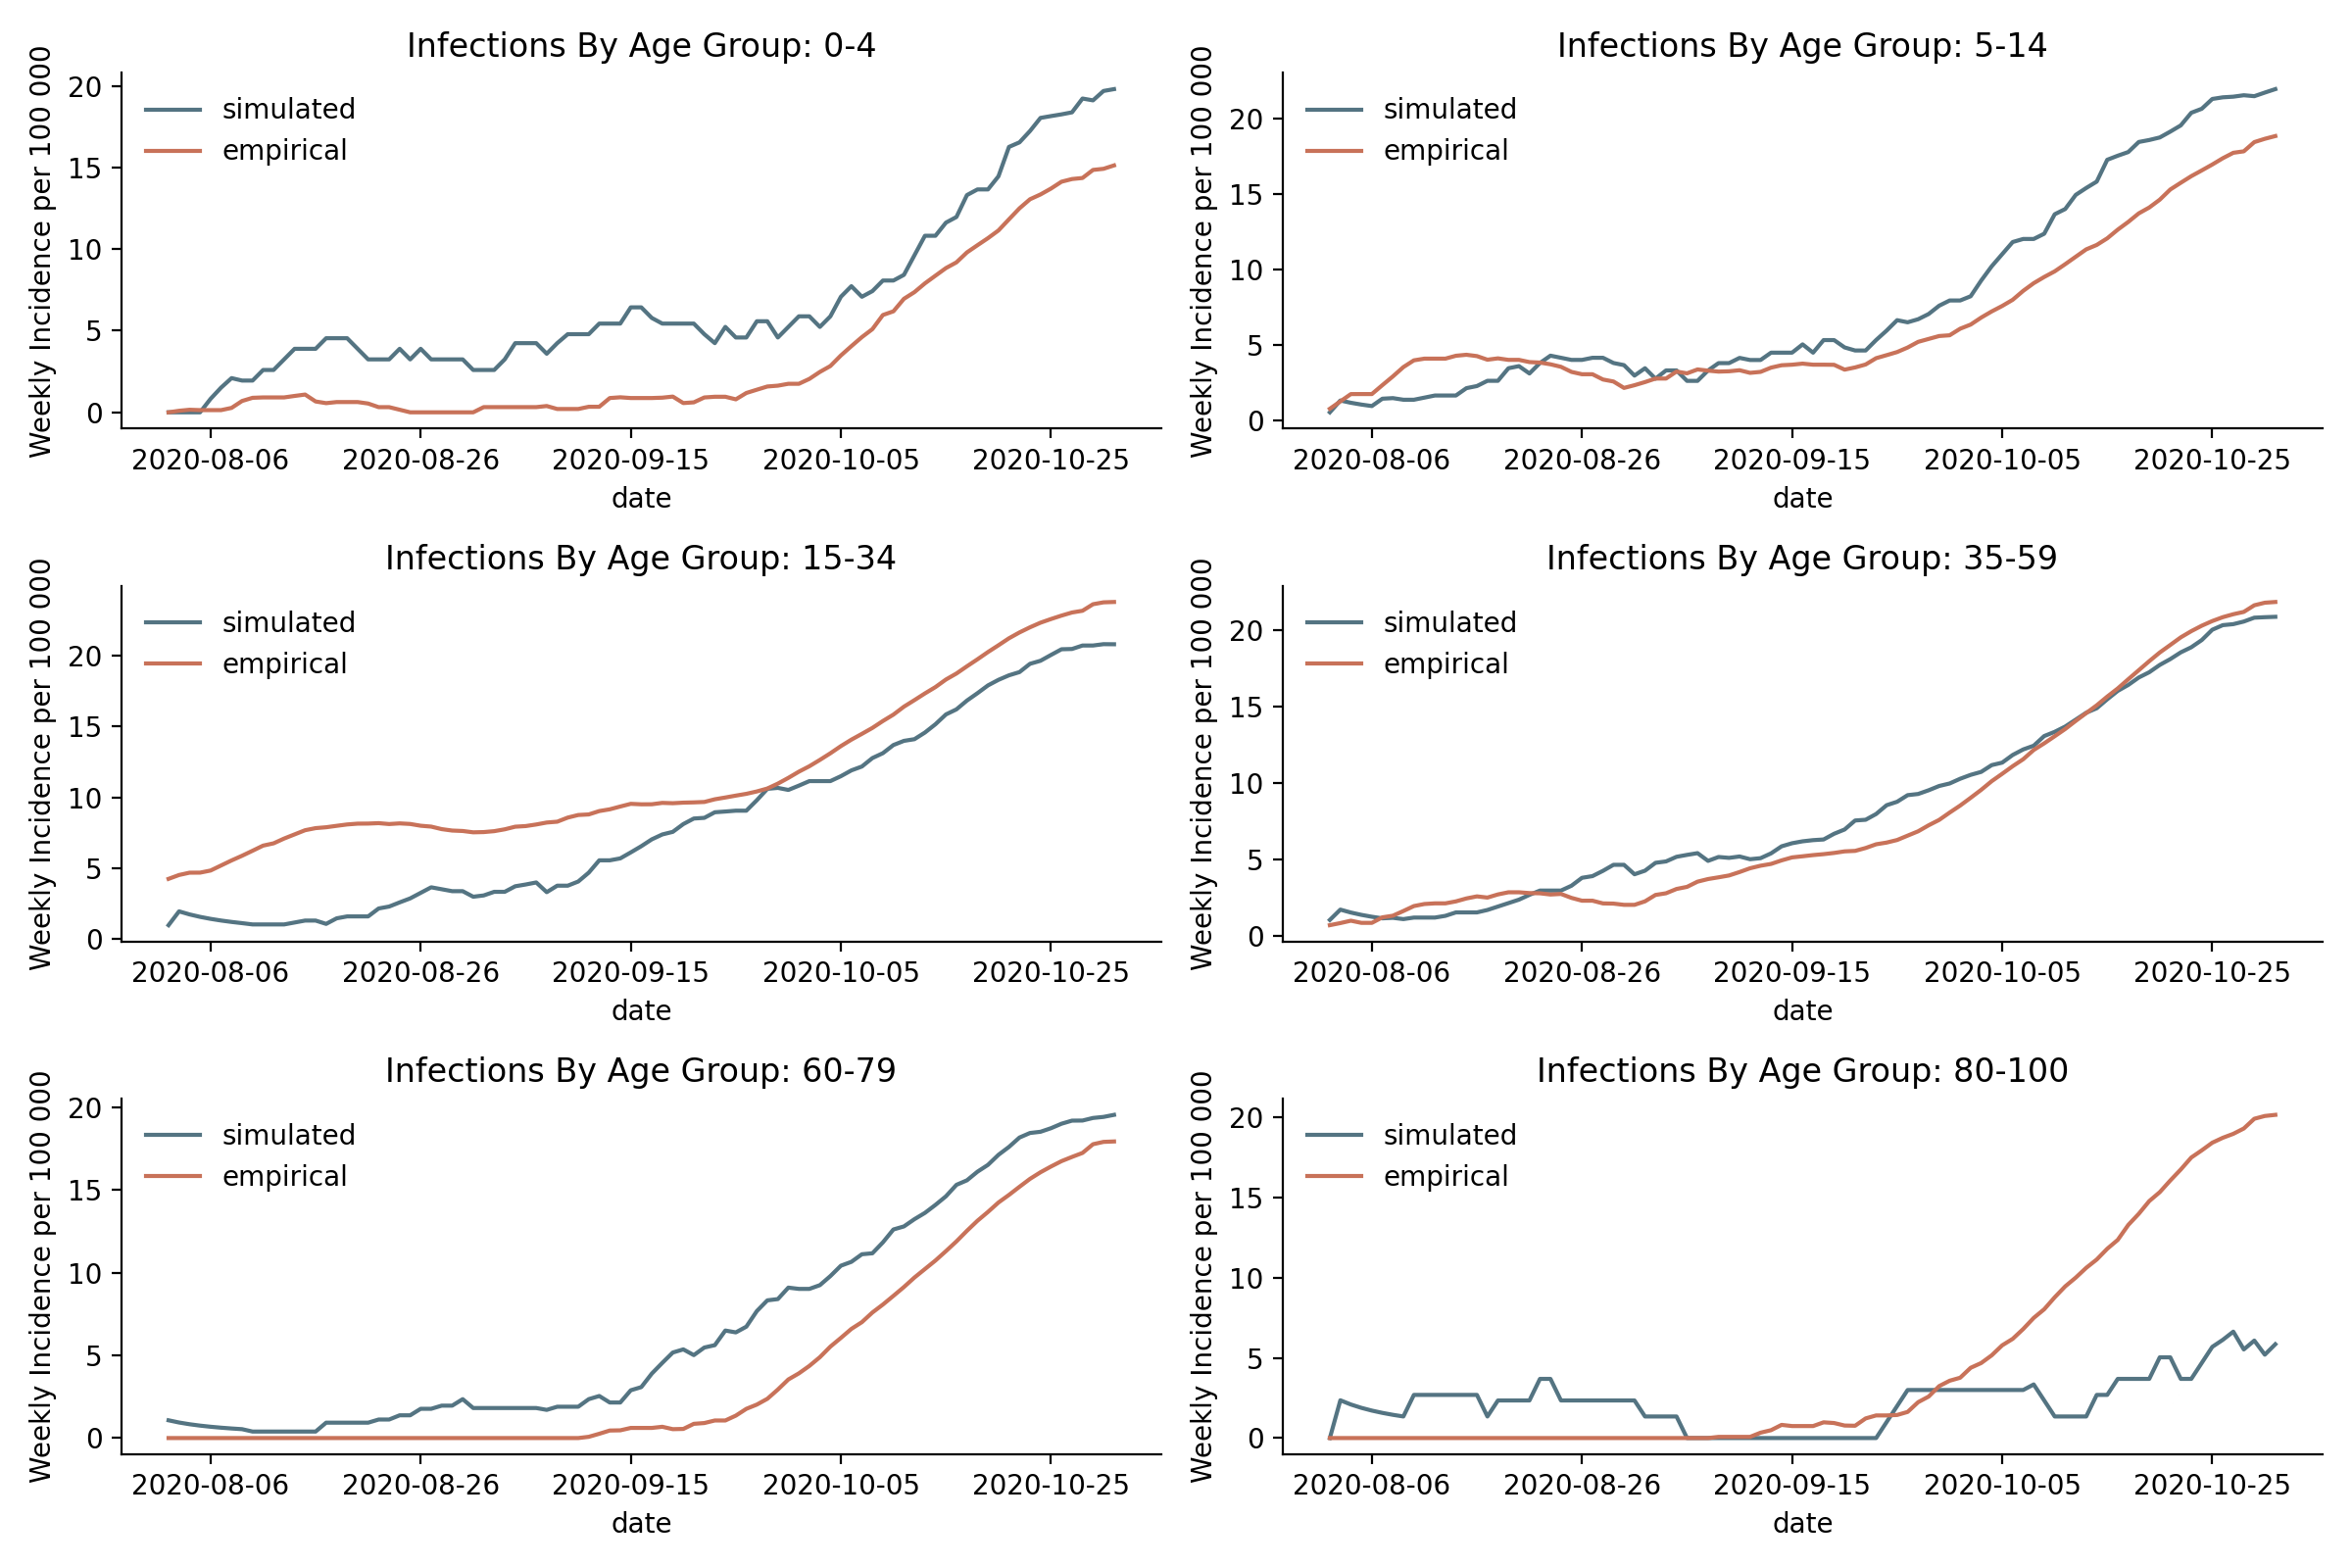
\includegraphics[width=\textwidth]{../figures/goodness_of_fit_by_age_group}
    \caption{Actual vs. simulated infection and fatality rates}
    \label{fig:goodness_of_fit}
\end{figure}


\subsection{Out-of-Sample Fit}

We can assess the out-of-sample fit by projecting the effect of the lockdown light and
comparing it to case numbers until now. It is important to note that this is not just a
simple extrapolation of a time trend because the lockdown light only started after the
estimation period. The out-of-sample fit can be assessed in
Figure~\ref{fig:out-of-sample-fit}.

\begin{figure}[!tp]
    \centering
    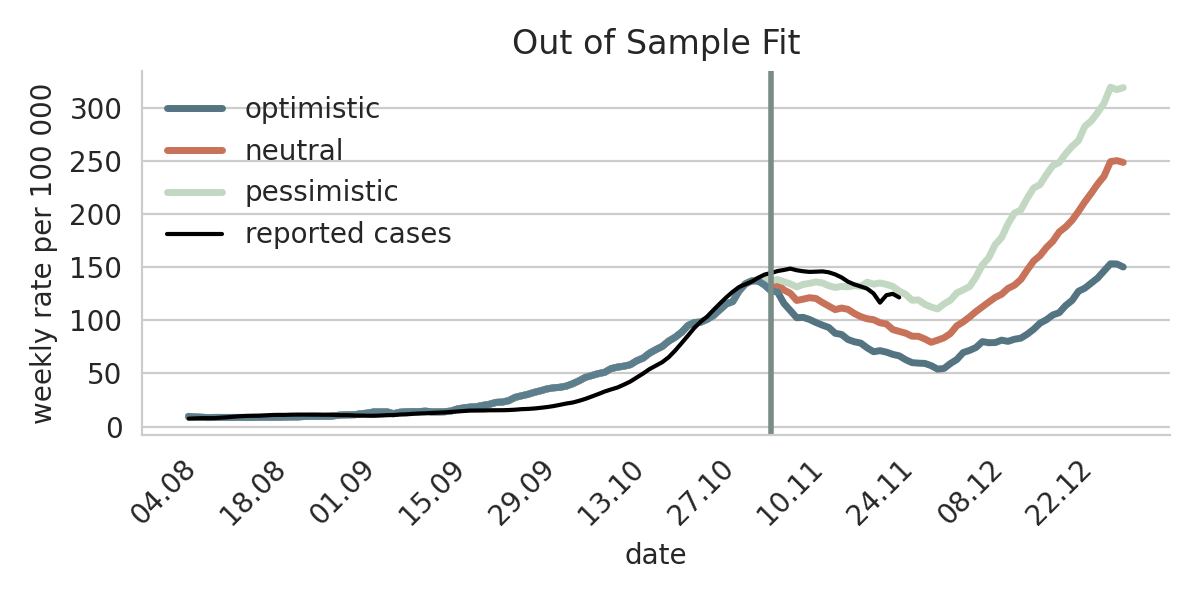
\includegraphics[width=\textwidth]{../figures/out_of_sample_validation}
    \caption{Projected effect of the lockdown-light}
    \label{fig:out-of-sample-fit}
\end{figure}

The model correctly predicts the effect of the lockdown light with reasonable accuracy.
In particular, the actual case numbers are between our neutral and pessimistic
projection. The plot also shows that ending the lockdown light as planned on November 30
would lead to an explosive growth in case numbers in all scenarios.
